\documentclass[11pt]{article}
\usepackage{enumerate}
\usepackage{fullpage}
\usepackage{fancyhdr}
\usepackage{tikz}
\usepackage{amsmath, amsfonts, amsthm, amssymb}
\setlength{\parindent}{0pt}
\setlength{\parskip}{5pt plus 1pt}
\pagestyle{empty}

\def\indented#1{\list{}{}\item[]}
\let\indented=\endlist

\newcounter{questionCounter}
\newcounter{partCounter}[questionCounter]
\newenvironment{question}[2][\arabic{questionCounter}]{%
    \setcounter{partCounter}{0}%
    \vspace{.25in} \hrule \vspace{0.5em}%
        \noindent{\bf #2}%
    \vspace{0.8em} \hrule \vspace{.10in}%
    \addtocounter{questionCounter}{1}%
}{}
\renewenvironment{part}[1][\alph{partCounter}]{%
    \addtocounter{partCounter}{1}%
    \vspace{.10in}%
    \begin{indented}%
       {\bf (#1)} %
}{\end{indented}}

%%%%%%%%%%%%%%%%%%%%%%%%%%%%%%%%%%%%%%%%%%%%%%%%%%%%%%%%%%%
\newcommand{\myname}{Shashank Singh}
\newcommand{\myandrew}{sss1@andrew.cmu.edu}
\newcommand{\myclass}{21-484A Graph Theory}
\newcommand{\myhwnum}{1}
\newcommand{\duedate}{Wednesday, February 1, 2012}
%%%%%%%%%%%%%%%%%%%%%%%%%%%%%%%%%%%%%%%%%%%%%%%%%%%%%%%%%%%

\begin{document}
\thispagestyle{plain}

{\Large Homework \myhwnum} \\
\myclass \\
Name: \myname \\
Email: \myandrew \\
Due: \duedate

%NOT DONE
\begin{question}{Problem 1} Let $G$ be a graph with at least $3$ vertices.
\begin{enumerate}[(a)]
%DONE
\item Suppose $G$ contains two distinct vertices $u$ and $v$ such that
$G_u := G - \{u\}$ and $G_v - \{v\}$ are both connected. Since $G$ contains at
least $3$ vertices, $G$ contains some vertex $t \neq u, v$. Since $G_u$ is
connected, for every vertex $s \neq u$ in $G$, there is a $s-t$ path in $G_u$.
Since $G_u$ is a subgraph of $G$, that $s-t$ path is also in $G$. Since $G_v$
is connected, there exists a $t-u$ path in $G_v$, and, since $G_v$ is a
subgraph of $G$, that $t-u$ path is also in $G$. Thus, for every vertex $r$ in
$G$, there is a $r-t$ path in $G$. Thus, for every pair of vertices $(r,s)$ in
$G$ reversing a $r-t$ path, removing $t$, and appending it to a $s-t$ path
gives a $s-r$ walk. Since, as shown in class, every $s-r$ walk contains a
$s-r$ path, $G$ has a $s-r$ path. Thus, since $s$ and $r$ are arbitrary nodes
in $G$, $G$ is connected. \qquad $\blacksquare$ \\

%DONE
\item Suppose, for sake of contradiction, that there exists a connected graph
$G$ such that, for every two distinct vertices $u$ and $v$ in $G$, $G- \{u\}$
and
$G - \{v\}$ are disconnected. In particular, let $G$ be a minimal such graph,
with respect to the number of nodes in $G$. It can be shown, by enumerating
all graphs on $1$ and $2$ nodes that no such graphs exists on fewer than $3$
nodes. Let $t$ be a vertex in $G$, and let $H = G - \{t\}$. Since $H$ is
disconnected, it has (at least) two distinct connected components, $K$ and
$L$. Since $K$ and $L$ each have fewer vertices than $G$, they each must have
$2$ vertices, $a$ and $b$ in $K$, and $c$ and $d$ in $L$, such that
$K - \{a\}$, $K - \{b\}$, $L - \{c\}$, and $L - \{d\}$ are each connected
(we can exclude the case that $K$ or $L$ has only one vertex, as, in this
case, removing that vertex would not cause $G$ to be disconnected).
Let $u = a$ if $at$ is not an edge in $G$, and let $u = b$ otherwise, and let
$v = c$ if $ct$ is not an edge in $G$, and let $v = d$ otherwise. Then,
$G - \{u\}$ and $G - \{v\}$ are both connected, contradicting the choice of
$G$. Therefore, for every connected graph $G$, there exist two distinct
vertices $u$ and $v$ in $G$ such that $G - \{u\}$ and $G - \{v\}$ are
connected. \qquad $\blacksquare$ \\

%DONE
\item Let $V = \{1, 2, 3, 4\}$, let $E = \{\{1, 2\}, \{2, 3\}, \{3, 4\}\}$,
and let $G = (V, E)$ (the graph pictured below).
\begin{center}
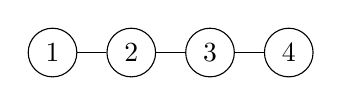
\begin{tikzpicture}
  [scale=1,auto=center,every node/.style={draw,circle}]
  \node (n1) at (1,1)  {1};
  \node (n2) at (2,1) {2};
  \node (n3) at (3,1)  {3};
  \node (n4) at (4,1)  {4};
  \foreach \from/\to in {n1/n2,n2/n3,n3/n4}
    \draw (\from) -- (\to);
\end{tikzpicture}
\end{center}
Then, $G$ is a graph with at least four vertices, but,
for any three distinct vertices $u, v,$ and $w$, since either $u, v$, or $w$
must be in $\{2, 3\}$, one of $G - \{u\}$, $G - \{v\}$, or $G - \{w\}$ is
disconnected. Thus, the statement in question is false. \qquad $\blacksquare$
\end{enumerate}
\end{question}

%DONE
\begin{question}{Problem 2} Suppose $G$ is a disconnected graph. Let $u$ and
$v$ be vertices in $G$. If $u$ and $v$ are in different connected components
of $G$, then $uv$ is not an edge in $G$, so that $uv$ is an edge in $\overline{G}$
and thus there exists a $uv$ path in $\overline{G}$. If $u$ and $v$ are in the same
connected component of $G$, then there exists a vertex $t$ in $G$ such that
$t$ is in a different connected component than $u$ and $v$ (if this were not
the case, then every vertex in $G$ would be in the same connected component of
$G$, so that $G$ would be connected). Since $t$ is in a different connected
component of $G$ than $u$ and $v$, $ut$ and $tv$ are not edges in $G$, so that
they are edges in $\overline{G}$. Therefore, $u,t,v$ is a $uv$ path in $\overline{G}$.
Thus, if $G$ is not connected, then $\overline{G}$ is connected, so that, for all
graphs $G$, either $G$ or $\overline{G}$ is connected. \qquad $\blacksquare$
\end{question}

%DONE
\begin{question}{Problem 3}
Let $V = \{1, 2\}$, let $E = \emptyset$, and let $G = (V, E)$ (the graph
pictured below).
\begin{center}

\begin{tikzpicture}
  [scale=1,auto=center,every node/.style={draw,circle}]
  \node (n1) at (1,1)  {1};
  \node (n2) at (2,1) {2};
\end{tikzpicture}
\end{center}
Then, for all vertices $u$ and $v$ in $G$, deg$(u) +$
deg$(v) = 0 \geq n - 2$. However, $G$ is disconnected. Thus, the condition in
question is sharp. \qquad $\blacksquare$
\end{question}

%DONE
\begin{question}{Problem 4}
Let $G$ be a graph, and let $u$ and $v$ be verticea in $G$. Suppose $u$ and
$v$ are in the same connected component $H$ if $G$. Then, if $u$ and $v$ are
not connected, then $H$ is not connected, contradicting the definition of $H$
as a connected component. Thus, if $u$ and $v$ are in the same connected
component of $G$, then $uRv$. Suppose, on the other hand, that $u$ and $v$ are
not in the same connected component of $G$, but $u$ and $v$ are connected. Let
$H$ be a connected component of $G$ containing $u$. If $v$ is not in $H$,
then, if $K$ is the graph created by adding the vertex $v$ and the edge $uv$
to $H$, the $H$ is a proper subgraph of $H$, which is a connected subgraph of
$G$, contradicting the maximality of $H$ as a connected component. Therefore,
if $uRv$, then $u$ and $v$ are in the same connected component of $G$, then
$u$ and $v$ are connected. Thus, two vertices in $G$ are in the same connected
component if and only if they are connected, so the equivalence classes of $R$
are the connected components of $G$. \qquad $\blacksquare$

\end{question}

%NOT DONE
\begin{question}{Problem 5}
\begin{enumerate}[(a)]
%DONE
\item The graph pictured below has the given degree sequence, so that the
given degree sequence is graphical.
\begin{center}
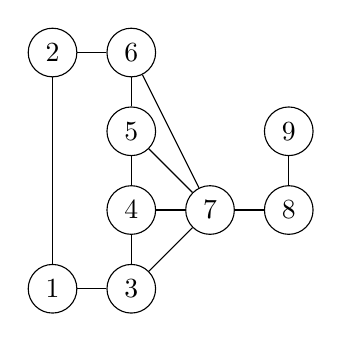
\begin{tikzpicture}
  [scale=1,auto=center,every node/.style={draw,circle}]
  \node (n1) at (1,1)  {1};
  \node (n2) at (1,4)  {2};
  \node (n3) at (2,1)  {3};
  \node (n4) at (2,2)  {4};
  \node (n5) at (2,3)  {5};
  \node (n6) at (2,4)  {6};
  \node (n7) at (3,2)  {7};
  \node (n8) at (4,2)  {8};
  \node (n9) at (4,3)  {9};
  \foreach \from/\to in {n1/n2,n2/n6,n1/n3,n3/n4/,n4/n5,n5/n6,n3/n7,n4/n7,n5/n7,n6/n7,n7/n8,n8/n9}
    \draw (\from) -- (\to);
\end{tikzpicture}
\end{center}

%DONE
\item The graph pictured below has the given degree sequence, so that the
given degree sequence is graphical.
\begin{center}
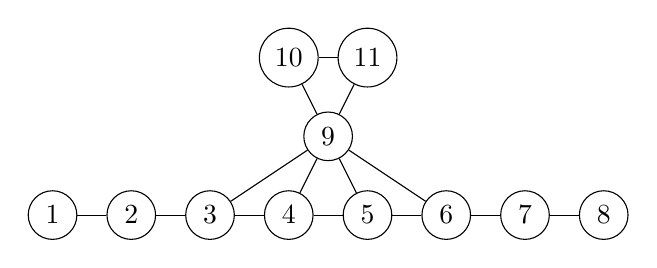
\begin{tikzpicture}
  [scale=1,auto=center,every node/.style={draw,circle}]
  \node (n1) at (1,1)  {1};
  \node (n2) at (2,1)  {2};
  \node (n3) at (3,1)  {3};
  \node (n4) at (4,1)  {4};
  \node (n5) at (5,1)  {5};
  \node (n6) at (6,1)  {6};
  \node (n7) at (7,1)  {7};
  \node (n8) at (8,1)  {8};
  \node (n9) at (4.5,2)  {9};
  \node (n10) at (4,3) {10};
  \node (n11) at (5,3) {11};
  \foreach \from/\to in {n1/n2,n2/n3,n3/n4,n4/n5,n5/n6,n6/n7,n7/n8,n3/n9,n4/n9,n5/n9,n6/n9,n9/n10,n9/n11,n10/n11}
    \draw (\from) -- (\to);
\end{tikzpicture}
\end{center}

%DONE
\item The graph pictured below has the given degree sequence, so that the
given degree sequence is graphical.
\begin{center}
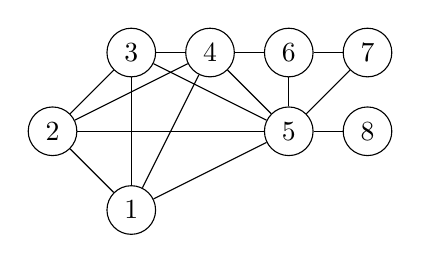
\begin{tikzpicture}
  [scale=1,auto=center,every node/.style={draw,circle}]
  \node (n1) at (2,1)  {1};
  \node (n2) at (1,2)  {2};
  \node (n3) at (2,3)  {3};
  \node (n4) at (3,3)  {4};
  \node (n5) at (4,2)  {5};
  \node (n6) at (4,3)  {6};
  \node (n7) at (5,3)  {7};
  \node (n8) at (5,2)  {8};
  \foreach \from/\to in {n1/n2,n2/n3,n1/n3,n2/n4,n3/n4,n1/n4,n4/n6,n1/n5,n2/n5,n3/n5,n4/n5,n5/n6,n5/n8,n5/n7,n6/n7}
    \draw (\from) -- (\to);
\end{tikzpicture}
\end{center}

%NOT DONE
\item The graph pictured below has the given degree sequence, so that the
given degree sequence is graphical.
\begin{center}
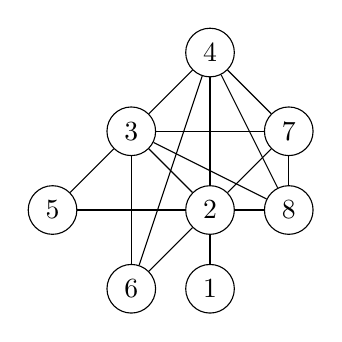
\begin{tikzpicture}
  [scale=1,auto=center,every node/.style={draw,circle}]
  \node (n1) at (3,1)  {1};
  \node (n2) at (3,2)  {2};
  \node (n3) at (2,3)  {3};
  \node (n4) at (3,4)  {4};
  \node (n5) at (1,2)  {5};
  \node (n6) at (2,1)  {6};
  \node (n7) at (4,3)  {7};
  \node (n8) at (4,2)  {8};
  \foreach \from/\to in {n1/n2,n2/n3,n2/n4,n2/n5,n2/n6,n2/n7,n2/n8,n3/n4,n3/n5,n3/n6,n3/n7,n3/n8,n4/n7,n7/n8,n4/n8,n4/n6}
    \draw (\from) -- (\to);
\end{tikzpicture}
\end{center}
\end{enumerate}
\end{question}

%DONE
\begin{question}{Problem 6} For $n = 1$, the only sequence of length $n$
obeying property (b) is the degree sequence of the graph with one vertex and
no edges, and is thus graphical. Suppose that, for some $n \in \mathbb{N}$,
all sequences of legraphical. Let $D = \{d_k\}_{1 \leq k \leq n + 1}$ be a sequence of
integers obeying properties (a), (b), and (c). Let
$E = \{e_k\}_{1 \leq k \leq n + 1}$ be a sequence that results from sorting
the terms of $D$ in descending order, so that $E$ also obeys properties (a),
(b), and (c). Let $F$ be the sequence
$f_2, f_3, \ldots, f_n = e_2 - 1, e_3 - 1, \ldots, e_{e_1} - 1,
e_{e_1 + 1} - 1, e_{e_1 + 2}, e_{e_1 + 3}, \ldots, e_n$, so that, as shown in
class, $E$ is graphical if and only if $F$ is graphical. Note that
\[\sum_{i = 1}^n f_i = \left( \sum_{i = 1}^{n + 1} e_i \right) - 2e_1,\]
so that, since $\sum_{i = 1}^{n + 1} d_i$ is even, $\sum_{i = 1}^n f_i$ is as
well, and thus $F$ obeys property (a). Suppose, for sake of contradiction
that $F$ did not obey property (b), so that it had some term $f_k$ such that
either $f_k > n - 1$ or $f_k < 0$. In the first case, since $f_k$ is an
element of $D$, which obeys property (b), $f_k = n$. However, since $E$ is
sorted in descending order, this would imply that $f_k \leq e_1 = n$, so that
$f_k = e_k - 1 \leq n - 1$, which is a contradiction. In the second case,
since $D$ obeys property (b), $f_k = -1$, as $e_k = 0$. Since $E$ obeys
property (c), this implies that $0 \leq e_1 \leq 1$. If $e_1 = 0$, then
$f_k = e_k \geq 0$, which is a contradiction. If $e_1 = 1$, then either
$e_2 = 0$, which would contradict the fact that $E$ obeys property (a), or
$e_2 = 1$, in which case either $k = 2$ and $f_k = 0$, or $k > 2$, in which
case $f_k = e_k \geq 0$; either is a contradiction. Thus, $F$ obeys property
(b). Suppose, for sake of contradiction, that $F$ does not satisfy property
(c), so that for some pair $(i, j)$ with $1 \leq i, j \leq n$ (without loss of
generality, $i < j$), $|f_i - f_j| > 1$. Since $E$ is sorted in descending
order and obey property (c), $0 \leq e_i - e_j \leq 1$. However, if
$f_j \neq e_j$, then $f_j = e_j - 1$, in which case, by construction of $F$,
$f_i = e_i - 1$, so that $f_i - f_j = e_i - e_j$, contradicting the fact that
$E$ obeys property (c), so that $F$ must also obey property (c).
Since $F$ is a sequence of integers of length $n$ obeying properties (a), (b),
and (c), by the induction hypothesis, $F$ is graphical, so that $E$ and thus
$D$ are graphical. By the Principle of Mathematical Induction, then, any
sequence of integers obeying properties (a), (b), and (c) is graphical. \qquad
$\blacksquare$
\end{question}
\end{document}
